% !TEX TS-program = Xelatex
% !TEX encoding = UTF-8 Unicode

\documentclass[UTF8]{ctexart}
\usepackage{amsmath}
\usepackage[bottom]{footmisc}
\usepackage{geometry}
\usepackage{pdfpages}
\usepackage{hyperref}
\usepackage{graphicx}
\usepackage{figsize}
\usepackage[separate-uncertainty = true,per-mode=symbol]{siunitx}
\usepackage{tabu}
\usepackage{wasysym}
\geometry{left=0.6in,right=0.6in,bottom=0.6in,top=0.6in}

\title{实验十八:弗兰克-赫兹实验}
\author{朱寅杰 1600017721}
\date{2018年3月16日}

\begin{document}
\maketitle
\setcounter{section}{18}
\subsection{Hg和Ar第一激发态的测量}
对于Hg管,管内温度调至\SI{176}{\degreeCelsius}。导流电压取为$U_{Kg1}=\SI{1.51}{\V}$,减速电压取为$U_{g2p}=\SI{2.06}{\V}$,测一条输出电流(经过放大器转化为电压信号)随扫描电压$U_{Kg2}$变化的伏安曲线。实验数据见数据页前两栏,所得图线见图1(a)。从图中读出几个电压峰值的位置分别在\SI{4.70}{\V}、\SI{9.51}{\V}、\SI{14.24}{\V}、\SI{19.17}{\V}、\SI{24.15}{\V}、\SI{29.20}{\V}处,各数据允差均取\SI{.05}{\V}。用Origin做最小二乘,得到斜率为\SI{4.896(30)}{\V},相关系数为\num{.99993}。合成入允差,得斜率为\SI{4.896(34)}{\V}。因此认为汞的第一激发态能级测得为\SI{4.90(3)}{\eV}。

对于Ar管,灯丝电压调至\SI{2.8}{\V},减速电压取为\SI{7.5}{\V},导流电压取为\SI{2.0}{\V},手动操作扫描电压$U_{Kg2}$,测一条输出电流(经过放大器转化为电压信号)随之变化的伏安曲线,数据见数据页第三栏,所得图线见图1(b)。从图中读出几个电压峰值的位置分别在\SI{17.7} {\V}、\SI{28.8}{\V}、\SI{40.2}{\V}、\SI{52.0}{\V}、\SI{64.9}{\V}、\SI{77.8}{\V}处。由于数据点比较稀疏,Ar管的电流值的弛豫时间也远比Hg管长,因此在找峰过程中判断各数据允差均取\SI{.5}{\V}。用Origin做最小二乘,得到斜率为\SI{12.017(198)}{\V},相关系数为\num{.99946}。合成入允差,得斜率为\SI{12.017(261)}{\V}。因此认为氩的第一激发态能级测得为\SI{12.0(3)}{\eV}。

\subsection{分析导流电压和减速电压对Ar管特性的影响}
分别控制减速电压$U_{g2p}$与导流电压$U_{Kg1}$,使用自动模式对Ar管的伏安特性进行快速扫描并作出图像。灯丝电压保持为\SI{2.8}{\V}不变,减速电压分别取\SI{7.5}{\V}、\SI{9.0}{\V}、\SI{6.0}{\V},导流电压分别取\SI{2.0}{\V}、\SI{1.2}{\V}、\SI{3.6}{\V},共测了五组数据(见数据页四至八列),分成两个控制变量序列作图,图线见图2(a)、(b)。从图2(a)中可见,减速电压越大,电流的峰越矮,同时也出现得越晚。这并不难理解,因为减速电压越大,要使电子能顺利到达阳极的加速电压的起点也就越大;并且在电流的谷的位置,减速电压越大电流也就被拦截得越小。从图2(b)中可见,导流电压越大,电流的峰越矮,这就比较匪夷所思。查实验记录,我应该没有把\SI{1.2}{\V}和\SI{3.6}{\V}的两组数据记反(因为是先测一组再测另一组的,手机视频的时间戳不会骗人),但也不能完全排除这种可能,需要再做一次实验确认一下到底是记反了还是规律本就如此。

\subsection{说明}
后面几幅图线均是使用样条函数连接的,所以数据点越稀疏的图线画出来越好看,像数据点很多的Hg管图线就很丑陋。

所用的Hg管的响应十分快,调节扫描电压后很快就能得到一个稳定的(转化为电压信号的)电流值。因此Hg管的数据点就可以取得很仔细,找峰时人的信心很足,所以估计出一个很小的允差;Ar管的响应就非常慢,特别是在电流急剧变化时,屏幕上的显示值会需要经过数分钟才能达到平衡值,并且弛豫的距离还很长,因此难以在“把握测量节奏”的同时很仔细地选取数据点,对测得的数据也没有什么信心,找峰时允差会估计得比较大。在手动测量图中可以看到有一两处有明显的卡顿,应该就是节奏不稳弛豫时间不同造成的不光滑。
\begin{figure}
  \centering
  \SetFigLayout{2}{1}
  \subfigure[Hg管的测量结果。横轴为扫描电压,纵轴为经过放大器转化为电压信号的电流强度。]{\includegraphics[width=\linewidth]{Hg.eps}}\\
  \subfigure[Ar管的测量结果。横轴为扫描电压,纵轴为电流强度。]{\includegraphics[width=\linewidth]{Ar.eps}}\\
  \caption{Hg管和Ar管的手动测量图线。从中找峰得到Hg和Ar能级的测量结果。}
\end{figure}

\begin{figure}
  \centering
  \SetFigLayout{2}{1}
  \subfigure[保持灯丝供电$U_F=\SI{2.8}{\V}$,导流电压$U_{Kg_1}=\SI{2.0}{\V}$不变,令减速电压$U_{g_2p}$取不同值所测得的一组特性曲线。]{\includegraphics[width=0.9\linewidth]{JIANSU.eps}}\\
  \subfigure[保持灯丝供电$U_F=\SI{2.8}{\V}$,导流电压$U_{g_2p}=\SI{7.5}{\V}$不变,令减速电压$U_{Kg_1}$取不同值所测得的一组特性曲线。]{\includegraphics[width=0.9\linewidth]{DAOLIU.eps}}
  \caption{使用自动模式对Ar管在不同的减速电压$U_{g_2p}$与导流电压$U_{Kg_1}$下的伏安特性曲线进行快速扫描测量。实验所用的Ar管装置在测电流时弛豫时间很长(特别是在电流变化较快时),而扫描的速度可达140bpm以上,因此快速扫描时得到的电流作为测量值远不准确,但仍可以作为趋势参考。如果能建立出这个弛豫的模型(比如知道是指数函数),那可以通过一定的变换操作从所得快速扫描数据中还原出电流的真实值来。}
\end{figure}

\includepdf{datalist.pdf}
\end{document} 